The problem of exploring an unknown territory is a fundamental problem in
robotics. The goal of exploration is to gain as much information as possible
of the environment within bounded time. 
Applications of efficient exploration include search and rescue \cite{Kitano99robocuprescue}, planetary exploration \cite{apostolopoulos2001robotic} and military uses \cite{hougen2000miniature}.
The most common approach to exploration is based on \emph{frontiers}. A frontier
is a segment that separates known (explored) regions from unknown regions. By
moving towards frontiers, robots can focus their motion on discovery of new
regions. Yamauchi
\cite{yamauchi_frontier-based_1997,yamauchi_frontier-based_1998} was the first
to show a frontier-based exploration strategy. His work led to many
others (e.g,
\cite{burgard05tro,lau_behavioural_2003,sawhney_fast_2009,burgard_collaborative_2000}).

Most frontier detection methods are based on edge detection and region
extraction techniques from computer vision. To detect frontiers, they
process the entire map data with every execution to the algorithm.
State-of-the-art frontier detection algorithms can take a number of seconds to run, even on powerful
computers. If a large region is explored, the robot actually has to wait in its
spot until the frontier detection algorithm terminates. Therefore, many
exploration implementations call the frontier detection algorithm only when the
robot arrives at its destination. 
 
This slows down the exploration process. It also can cause inefficiencies in the
exploration.
We present two examples:
First, consider a common \textit{single-robot case} (Figure~\ref{fig:single_example}),
where a robot exploring its environment detects a frontier and moves towards it (Figure~\ref{fig:single_1}).
Because of sensor coverage, the robot may in fact sense (and clear) all remaining unknown
area (Figure~\ref{fig:single_2}), but because it cannot call the
frontier-detection mechanism, it continues to move unnecessarily
(Figure~\ref{fig:single_3}). Similarly, consider a \textit{multi-robot case}
(Figure~\ref{fig:mutli_example}). Here, two robots,
 $R_1$ and $R_2$ which are located on bottom and top, respectively, 
are exploring the environment, from their initial locations (Figure~\ref{fig:multi_1}). 
One of the robots passes by a target assigned to the other, and thus clearing it
(Figure~\ref{fig:multi_2}).
But because the other robot cannot continuously re-detect frontiers, it unnecessarily continues
towards the covered target, instead of turning to more fruitful exploration targets.

\begin{figure}
 \centering
 \subfigure[ ] {
 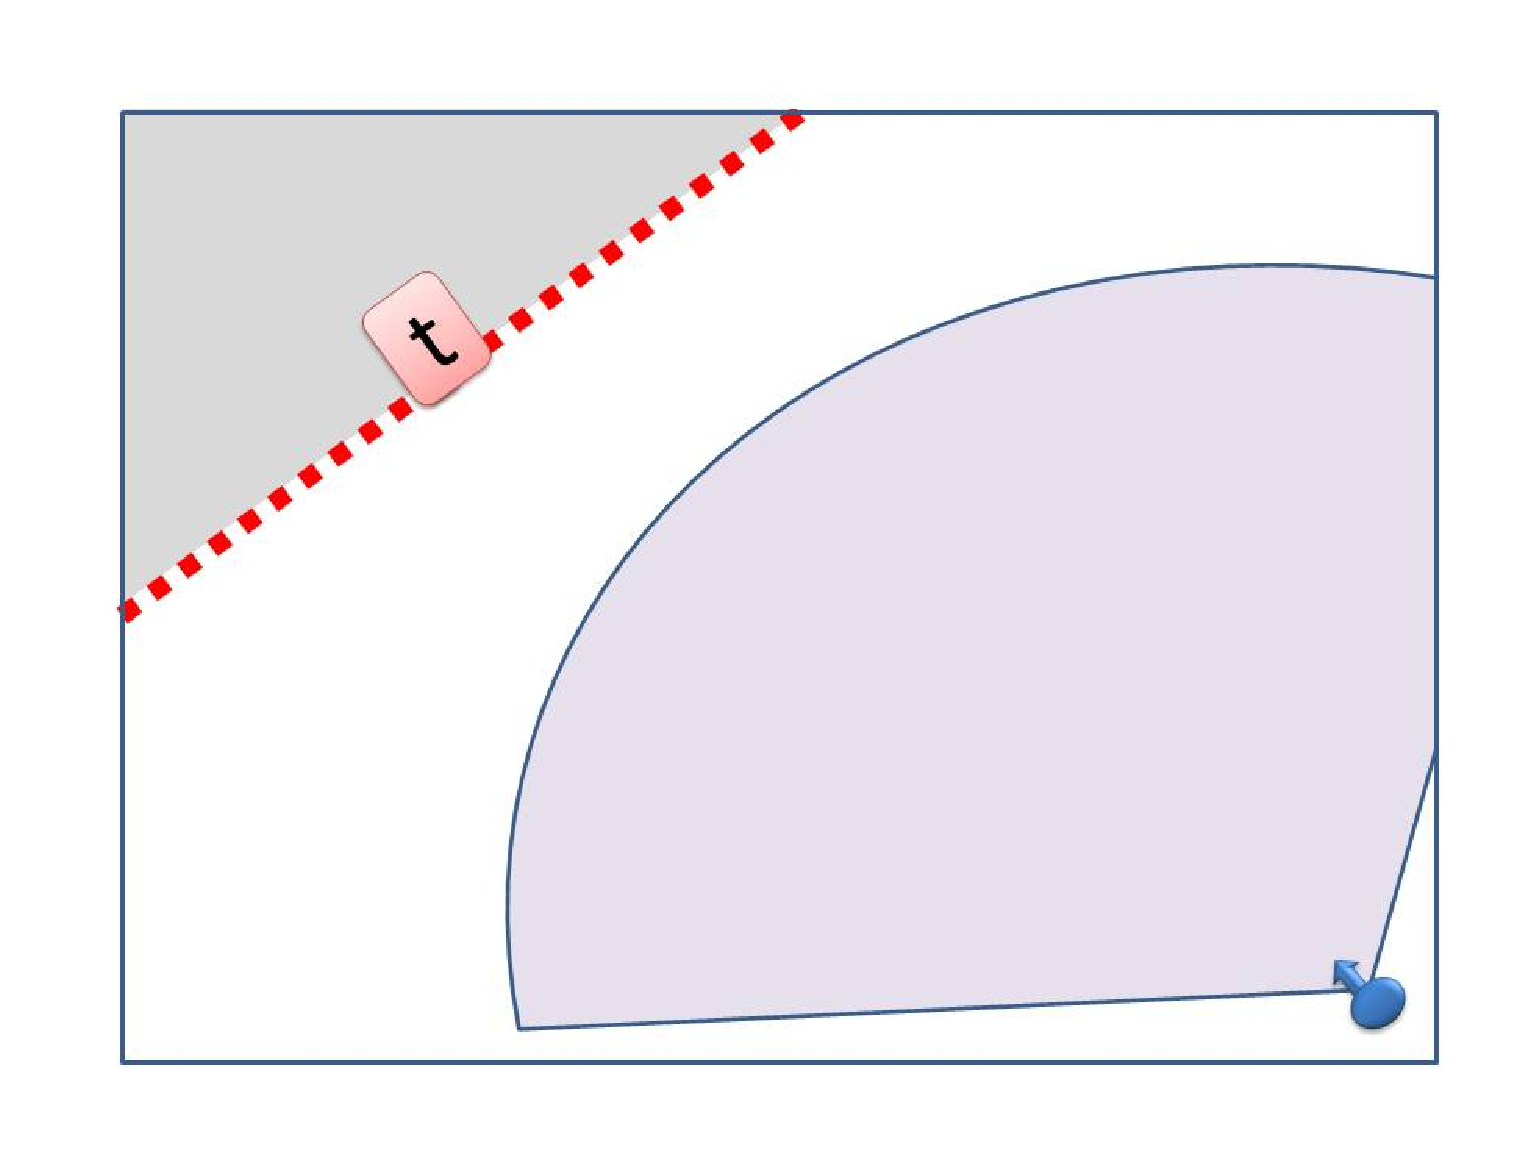
\includegraphics[width=0.3\columnwidth,keepaspectratio]{images/single_1}
 \label{fig:single_1}}
 \subfigure[ ] {
 \centering
 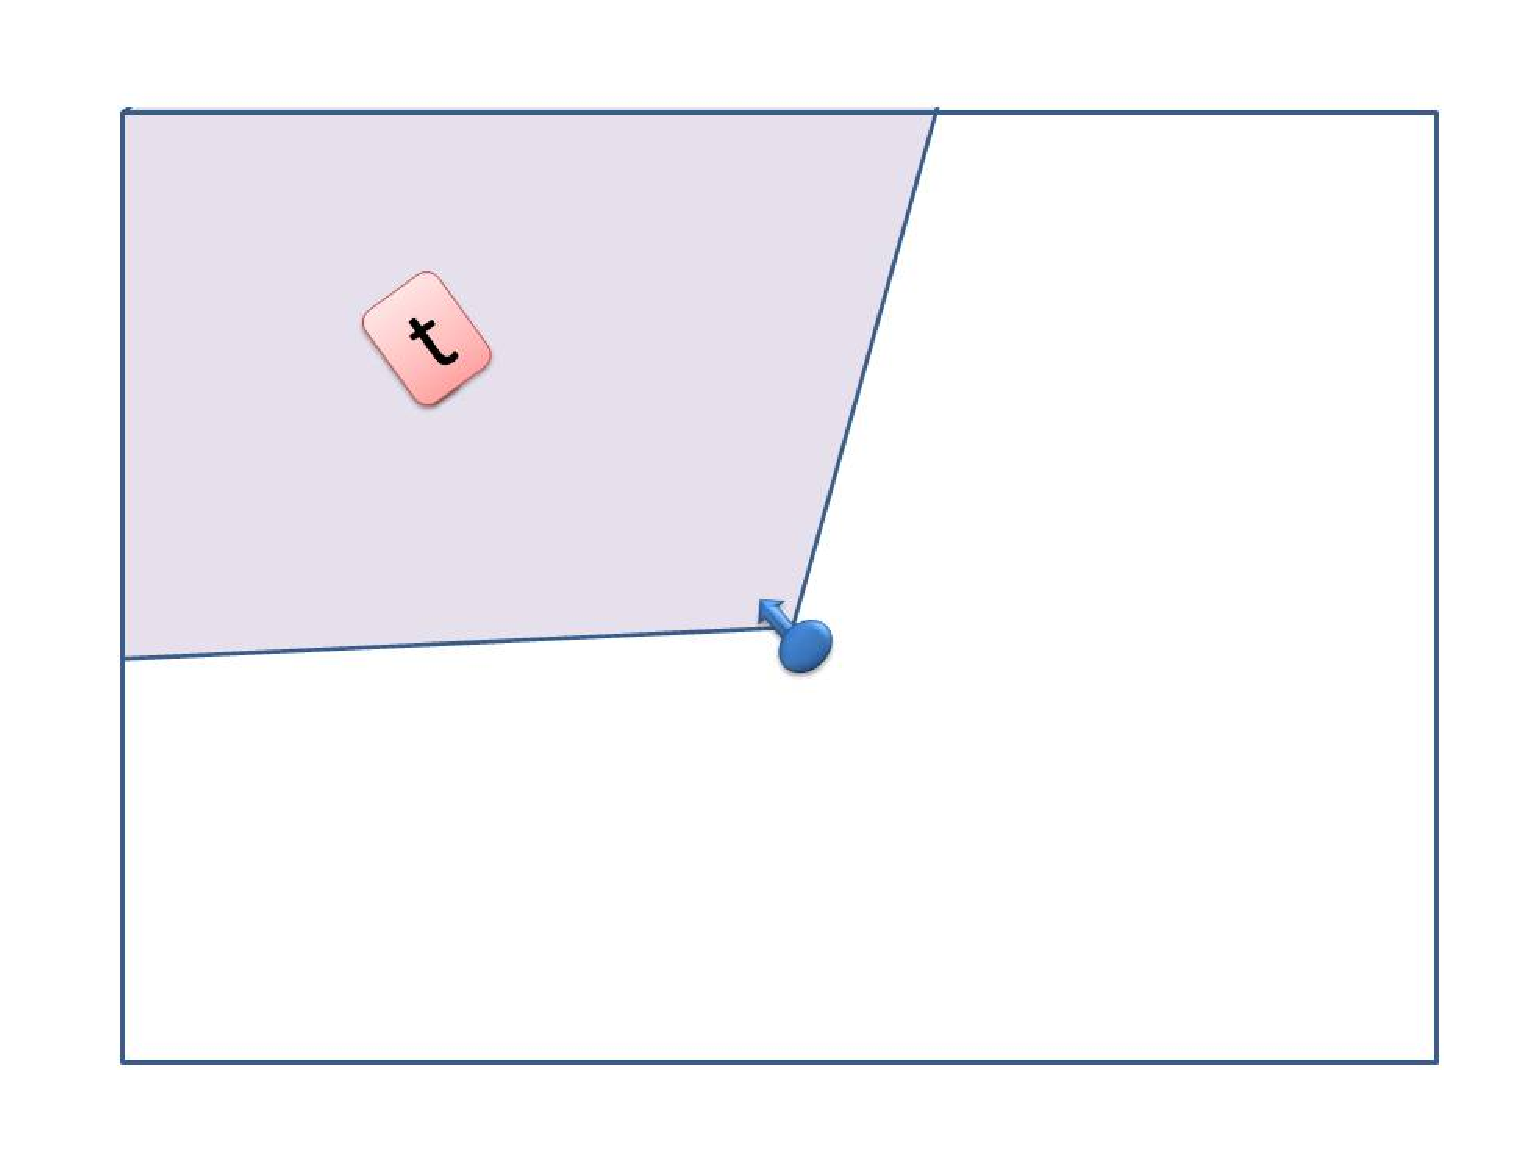
\includegraphics[width=0.3\columnwidth,keepaspectratio]{images/single_2}
 \label{fig:single_2}}
 \subfigure[ ] {
 \centering
 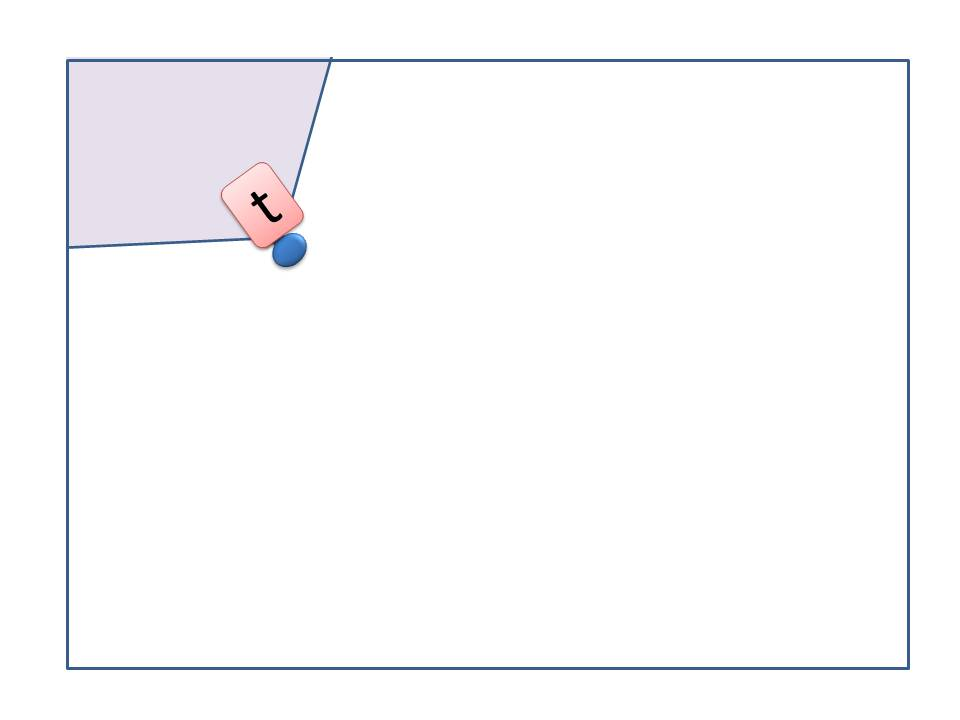
\includegraphics[width=0.3\columnwidth,keepaspectratio]{images/single_3}
 \label{fig:single_3}
 }
 \caption{A single-robot example. In 
 \ref{fig:single_1} the robot is heading towards the marked target on the frontier.  In 
 \ref{fig:single_2} the target and all of the remaining are covered by the robot's sensors, but because the robot does
  not re-detect frontiers, it continues to move.  In  \ref{fig:single_3} the robot has reached the frontier, unnecessarily.
 }
 \label{fig:single_example}
 
\end{figure}


\begin{figure}
 \centering
 \subfigure[] {
 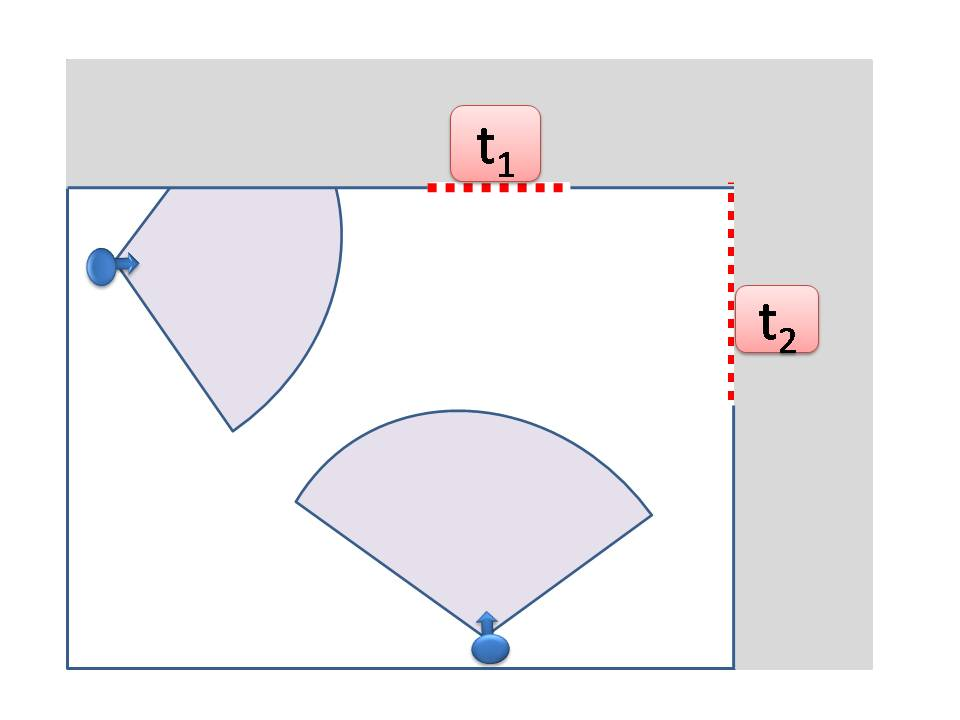
\includegraphics[width=0.45\columnwidth,keepaspectratio]{images/multi_1}
 \label{fig:multi_1}}
 \subfigure[] {
 \centering
 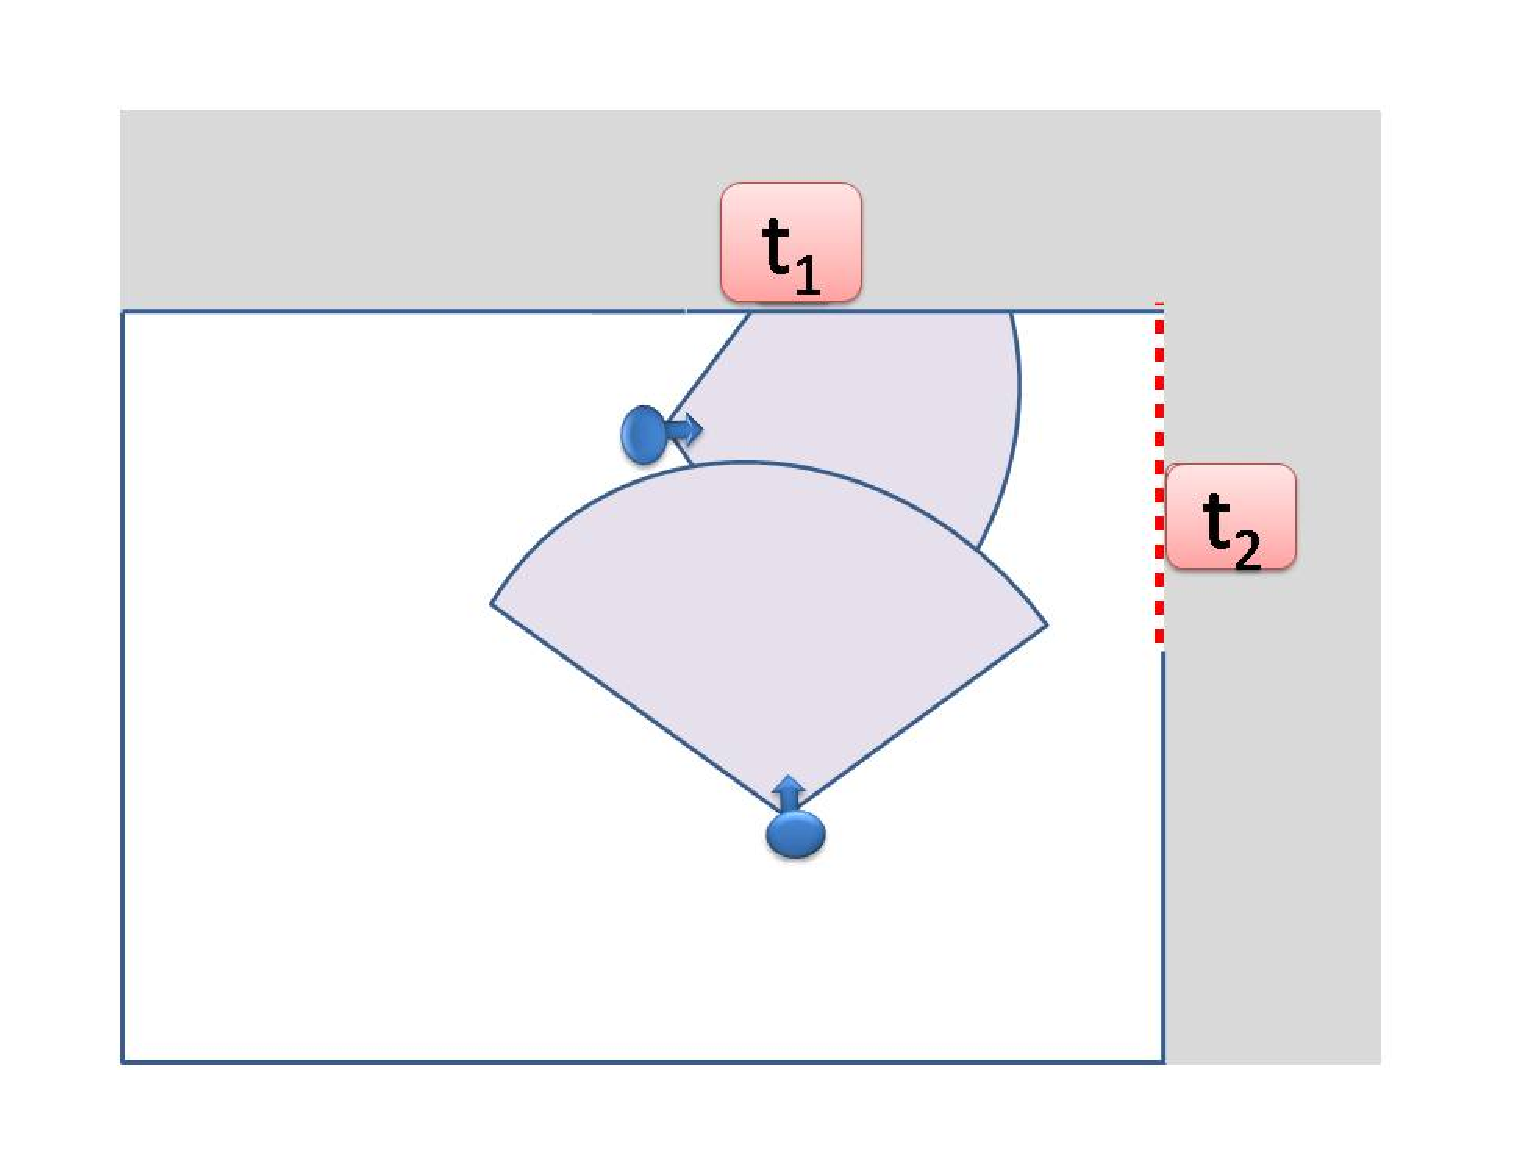
\includegraphics[width=0.45\columnwidth,keepaspectratio]{images/multi_2}
 \label{fig:multi_2}}
 \caption{A multi-robot example.  In~\ref{fig:multi_1}, the top robot ($R_2$) is heading towards the right target, $t_2$; the other robot ($R_1$) heads towards the top target $t_1$. In~\ref{fig:multi_2} $R_2$ has reached its target, clearing both $t_1$ and $t_2$, making $R_1$'s movements unnecessary.}
 \label{fig:mutli_example}
\end{figure}

In this thesis, we thus focus on significantly speeding up frontier detection.
We introduce four algorithms for fast frontier detection: 
The first, \WFD (Wavefront Frontier Detector) % (Section \ref{section:wfd})
is an iterative method that performs a graph-search over already-visited map
points. It builds on ideas suggested in earlier
work~\cite{Calisi:2007:MES:1291068.1291076} which were not evaluated as an
alternative to the edge-detection state-of-the-art. The key idea in \WFD is
that it does not scan the entire map, only the regions that have already been
visited by the robot.
However, as exploration progresses, the scanned area grows, and thus \WFD cannot
be expected to perform well in large areas.  Our second contribution is 
\FFD (Fast Frontier Detector), % (Section \ref{section:ffd}) is 
a novel approach for frontier detection which processes raw sensor readings,
and thus only scans areas that could contain frontiers. But because it works
with raw sensor data, it requires extending the mapper (SLAM) with additional
data-structures, so that frontiers are maintained
even when they are no longer within sensor range.
We describe these data-structures in detail, focusing on 
fast implementations.
Finally, we synthesized the different approaches of
\WFD and \FFD into two novel algorithms: \WFDINC and \WFDIP. Both algorithms
perform frontier detection on known regions but they differ from \WFD by
searching for frontiers only within the areas that were covered by the robot
sensors since last call.

\WFD and edge-detection methods use the occupancy grid
maintained by a SLAM mapper as a representation of the accumulated, processed sequence $\langle
O_0,\ldots,O_t\rangle$. They thus essentially ignore most of the sequence, and
act (mostly) on the latest observation of the grid $G_t$, as it integrates all
sensor readings up to time $t$. The edge detection method processes $G_t$ (the
entire occupancy grid at time $t$). The \WFD algorithm processes a subset,
starting with the cell indicated by $P_t$ (the latest robot position), within
$G_t$.  \FFD uses $R_t$ directly to detect current frontiers, and a modified
occupancy grid data structure to maintain/delete past frontiers.
We provide a theoretical complexity analysis for both algorithms and
in addition, \FFD is a novel approach and hence we proove its correctness. 
More definitions and terms related to the frontier detection problem can be
found in Section \ref{section:definitions}.

We provide a detailed evaluation of these algorithms, and contrast them 
with the state-of-the-art (\SOTA). % (in Section
% \ref{section:experimental_results}.
We examine their performance in different types of environments and two different
CPUs. We show that \WFD and \WFDINC are faster than \SOTA by 1--2 orders of
magnitude, and that \FFD and \WFDIP are faster than \WFD and \WFDINC by 1--2
orders of magnitude.  The results make it possible to execute real-time
frontier-detection on current-day robot CPUs, opening the way to novel
frontier-based exploration methods which were impractical until now.

\paragraph{List of Publications}
The work reported in this thesis has been published in the following
conferences:
\begin{itemize}
  \item \nobibentry{keidar2011arms}
  \item \nobibentry{keidar2012aamas}
\end{itemize}